% THIS IS SIGPROC-SP.TEX - VERSION 3.1
% WORKS WITH V3.2SP OF ACM_PROC_ARTICLE-SP.CLS
% APRIL 2009
%
% It is an example file showing how to use the 'acm_proc_article-sp.cls' V3.2SP
% LaTeX2e document class file for Conference Proceedings submissions.
% ----------------------------------------------------------------------------------------------------------------
% This .tex file (and associated .cls V3.2SP) *DOES NOT* produce:
%       1) The Permission Statement
%       2) The Conference (location) Info information
%       3) The Copyright Line with ACM data
%       4) Page numbering
% ---------------------------------------------------------------------------------------------------------------
% It is an example which *does* use the .bib file (from which the .bbl file
% is produced).
% REMEMBER HOWEVER: After having produced the .bbl file,
% and prior to final submission,
% you need to 'insert'  your .bbl file into your source .tex file so as to provide
% ONE 'self-contained' source file.
%
% Questions regarding SIGS should be sent to
% Adrienne Griscti ---> griscti@acm.org
%
% Questions/suggestions regarding the guidelines, .tex and .cls files, etc. to
% Gerald Murray ---> murray@hq.acm.org
%
% For tracking purposes - this is V3.1SP - APRIL 2009

\documentclass{acm_proc_article-sp}

\begin{document}

\title{02815 Web 2.0 and mobile interaction E11 - Assignment 1}
%\subtitle{[Extended Abstract]
%\titlenote{A full version of this paper is available as
%\textit{Author's Guide to Preparing ACM SIG Proceedings Using
%\LaTeX$2_\epsilon$\ and BibTeX} at
%\texttt{www.acm.org/eaddress.htm}}}
%
% You need the command \numberofauthors to handle the 'placement
% and alignment' of the authors beneath the title.
%
% For aesthetic reasons, we recommend 'three authors at a time'
% i.e. three 'name/affiliation blocks' be placed beneath the title.
%
% NOTE: You are NOT restricted in how many 'rows' of
% "name/affiliations" may appear. We just ask that you restrict
% the number of 'columns' to three.
%
% Because of the available 'opening page real-estate'
% we ask you to refrain from putting more than six authors
% (two rows with three columns) beneath the article title.
% More than six makes the first-page appear very cluttered indeed.
%
% Use the \alignauthor commands to handle the names
% and affiliations for an 'aesthetic maximum' of six authors.
% Add names, affiliations, addresses for
% the seventh etc. author(s) as the argument for the
% \additionalauthors command.
% These 'additional authors' will be output/set for you
% without further effort on your part as the last section in
% the body of your article BEFORE References or any Appendices.

\numberofauthors{8} %  in this sample file, there are a *total*
% of EIGHT authors. SIX appear on the 'first-page' (for formatting
% reasons) and the remaining two appear in the \additionalauthors section.
%
\author{
% You can go ahead and credit any number of authors here,
% e.g. one 'row of three' or two rows (consisting of one row of three
% and a second row of one, two or three).
%
% The command \alignauthor (no curly braces needed) should
% precede each author name, affiliation/snail-mail address and
% e-mail address. Additionally, tag each line of
% affiliation/address with \affaddr, and tag the
% e-mail address with \email.
%
% 1st. author
\alignauthor
Corneliu Sugar\\%\titlenote{Dr.~Trovato insisted his name be first.}\\
       \affaddr{Technical University of Denmark}\\
       \email{s111023@student.dtu.dk}
% 2nd. author
\alignauthor
S\o ren Ulrikkeholm\\%\titlenote{The secretary disavows
%any knowledge of this author's actions.}\\
       \affaddr{Technical University of Denmark}\\
       \email{s112460@student.dtu.dk}
}
% There's nothing stopping you putting the seventh, eighth, etc.
% author on the opening page (as the 'third row') but we ask,
% for aesthetic reasons that you place these 'additional authors'
% in the \additional authors block, viz.
\additionalauthors{Additional authors: John Smith (The Th{\o}rv{\"a}ld Group,
email: {\texttt{jsmith@affiliation.org}}) and Julius P.~Kumquat
(The Kumquat Consortium, email: {\texttt{jpkumquat@consortium.net}}).}
\date{30 July 1999}
% Just remember to make sure that the TOTAL number of authors
% is the number that will appear on the first page PLUS the
% number that will appear in the \additionalauthors section.

\maketitle
\begin{abstract}
(SU)
This report covers the work that was performed for solving assignment 1 in the course Web 2.0 and mobile interaction.
The report includes an analysis of which web 2.0 architectures have been applied by Zynga and LinkedIn, how they are profiting and how they could improve their services.
Furthermore, the report describes the different techniques used for mining and representing data from Twitter in interesting ways, and also attempts to make some analysis based on the data.
\end{abstract}

% A category with the (minimum) three required fields
%\category{H.4}{Information Systems Applications}{Miscellaneous}
%A category including the fourth, optional field follows...
%\category{D.2.8}{Software Engineering}{Metrics}[complexity measures, performance measures]

\terms{Data Mining}

\keywords{Web 2.0, Twitter, Python, Basemap, NetworkX} % NOT required for Proceedings

\section{Design Patterns}
\subsection{Zynga}

\subsection{LinkedIn (SU)}
The professional social network extensively uses declarative living and tag gardening as a pattern for offering a service of great relevance to their users. Its users provide vast amounts of information about themselves and their professional lives which LinkedIn in turn uses to suggest people that could be part of a person�s network, and display other types of content that could be of interest to the user. In this way LinkedIn utilizes its community to let users both connect with friends and establish new professional contacts, and also provides to possibility for users to build conversations either via personal messages of status updates.

In addition to creating an interesting service, LinkedIn also uses the information it mines to monetize from their product by selling advertisements to recruiters and companies interested in hiring specific types of people.

LinkedIn could, and perhaps already is, using the concept of curating identity to provide a more vertical experience in which professional and academic interests can be explored and improved.

\section{Networks (SU)}
As the original task, that asks that two users with each 2000 followers, proved to be too much to handle for the Twitter API, the task was re-formulated to use users with approximately 200 friends and followers each.

To make the results a little more relevant we chose to use S\o ren Ulrikkeholm (@sorenu, 114 friends, 25 followers) and an African male with approximately the same stats, i.e. age, interests (IT), and number of friends and followers. We were able to find a Twitter user with the screen name @vincente\_shiala who fit the description.

The first step in collecting information about each user is to make a script that collects all the friend and follower ids of a user, and then goes on to collect all of the friend ids of each of those users - note that we get the friend ids only in order to limit the number of requests we have to make later. Then we collect detailed information for each of the friends and followers. We are particularly interested in the location information which we will be using later.

The results are stored in a Redis database, so that we do not have to repeat the queries each time we want to use the data.

Most of the Twitter and Redis logic is given to us through the twitter\_\_util module from MTSW.

\begin{figure}
\centering
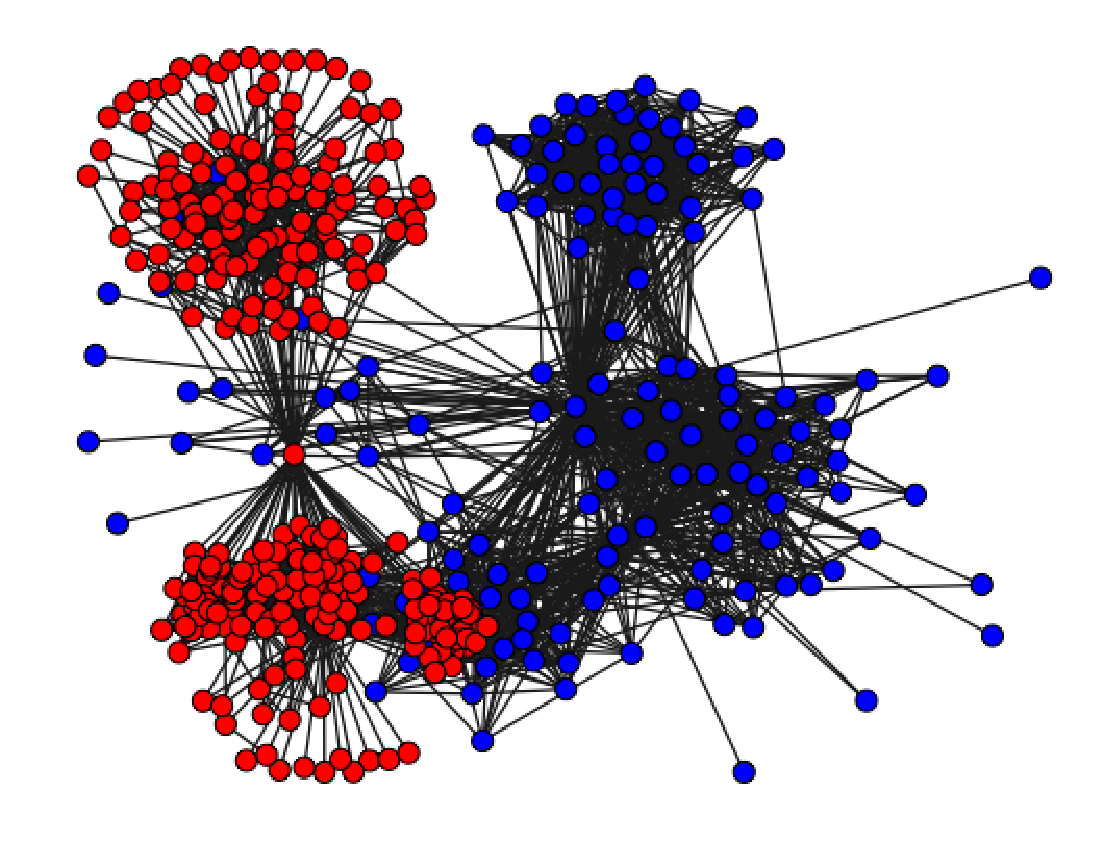
\includegraphics[scale=0.50]{eu_af_graph.eps}
\caption{A graph representing two twitter users' connections and how the connections are connected. Red is @vincente\_shiala - blue is @sorenu. NB: the red and blue graphs are not actually connected, but it looks cool when they are presented like this.}
\label{euafgraph}
\end{figure}

The data that we collect with the script can be represented in graphs by using the networkx Python library as shown in figure \ref{euafgraph}. It is interesting how both users' connections seem to be highly clustered. Especially @vincente\_shiala's connection are very distinctly divided into to clusters, with @vincente\_shiala acting as the global bridge between the two worlds.

\section{Geocoding (SU)}
The next step in the process of representing Twitter users on a map is to collect geographical data about the location of each user in our database.

To do this we firstly need some extra information about the users in our database in addition to their friend and follower ids. The getUserInfo method in the twitter\_\_util module lets us extract a vast amount of data, including location, for a list of user ids that we provide for it. Using this method we harvest location data for all of the users we are interested in, i.e. the friends and followers of our main user, and the friends of all of those users.

Now the locations need to be converted into longitudes and latitudes. The Bing Maps API allows you to query a location and have its coordinates returned along with a parameter stating the certainty of the result. In our script we only store the results with high certainty in our Redis database using the location name as the key. To decrease the necessary number of queries, we normalize the locations before querying by turning them all into lower case and checking the database if the location already exists before querying.

Since Twitter users tend to state strange locations it's important that the script is able handle bad responses from the Bing service.

\section{Mapping I (SU)}
As Twitter is a service very much about reaching the most amount of people, we decided to define "most important contacts" as the contacts that have the highest amount of followers.

To extract the top 20 users among the main user's friends and followers we use Redis' built-in set operations to do a union of the friends and followers which we turn into a dictionary with user\_id as the key and the number of followers as the value. We then turn the dictionary into a sorted list based on the values and extract the first twenty entries.

We then want to create a static Google map with the connections between the main user and his top twenty connections. To do this, we make use of the location and position data that we collected in the previous task. The Google maps API lets us draw paths on maps by calling the API with a URL containing an arbitrary number of path parameters. We create this URL based on the location and position information.

\begin{figure}
\centering
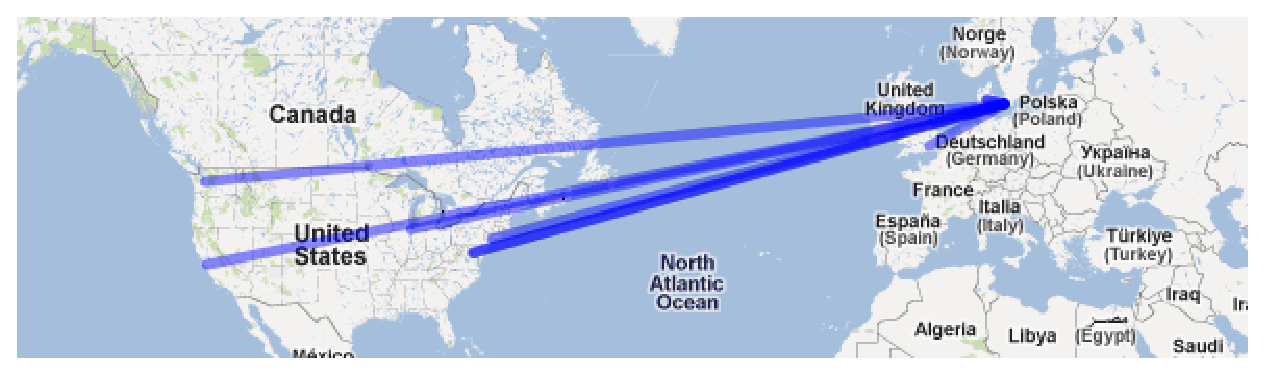
\includegraphics[scale=0.30]{g_maps.eps}
\caption{@sorenu's top twenty connections.}
\label{gmaps}
\end{figure}

When we open the URL we get the result as seen in figure \ref{gmaps}.


\begin{figure}
\centering

\includegraphics[scale=0.50]{tweet.eps}
\caption{The latest tweet from @vincente\_shiala.}
\end{figure}

\end{document}
